\documentclass{beamer}

\usetheme[progressbar=frametitle]{metropolis}

\usepackage{booktabs}
\usepackage[scale=2]{ccicons}
\usepackage{pgfplots}
\usepgfplotslibrary{dateplot}
\usepackage{xspace}
\newcommand{\themename}{\textbf{\textsc{metropolis}}\xspace}
\usepackage{listings}

\begin{document}

    \title{GitHub Kata}
    \author{Michell Pineda \\ 
            Julian Arango}
    \date{15 de Febrero de 2016}
    \frame{ \titlepage }

    \frame{
    \frametitle{Tabla de contenidos}

    \begin{enumerate}
        \item Diferencia entre Git y GitHub
 	    \item Servidores de repositorios Git
        \item Instalar Git
        \item C\'omo crear un repositorio?
	   \item Los tres estados

	  %\item Principales conceptos
        \item C\'omo compartir un repositorio?
        \item Committing, Pull y Push
        \item C\'omo crear un Brach?
        \item Merging
    \end{enumerate}
}

    \begin{frame}[fragile]
    \frametitle{Diferencia entre Git y Github}
        Git es un sistema de control de versiones distribuido, diseñado por
        Linus Torvalds, inicialmente para satisfacer las necesidades del
        Kernel de Linux, tras romper relaciones con la empresa que desarrollo
        su anterior herramienta (Bitkeeper).



Y qu\'e es Github? Es un hosting online para alojar repositorios que usan Git para el manejo del c\'odigo fuente.


\begin{figure}[t]
        \centering
        
\includegraphics[width=0.5\textwidth]{Images/1.png}
\end{figure}


%Por tanto Git es algo m\'as general que nos ayuda a controlar el estado de un proyecto, Github es un sitio que usa Git en su funcionamiento.

\end{frame}

    \frame{
\frametitle{Servidores de repositorios Git}

%Con Git instalado en nuestro computador tendremos un control de versiones con toda la funcionalidad, pero si nuestro proposito es compartir el c\'odigo con otras personas, debemos crear un repositorio en un servidor.

Algunos de ellos son:
\begin{itemize}
\item GitHub (Lo veremos m\'as detallado)
\item BitBucket
\item GitLab
\item Cloud Source Repositories (Beta)
\end{itemize}

\begin{figure}[t]
    \centering
    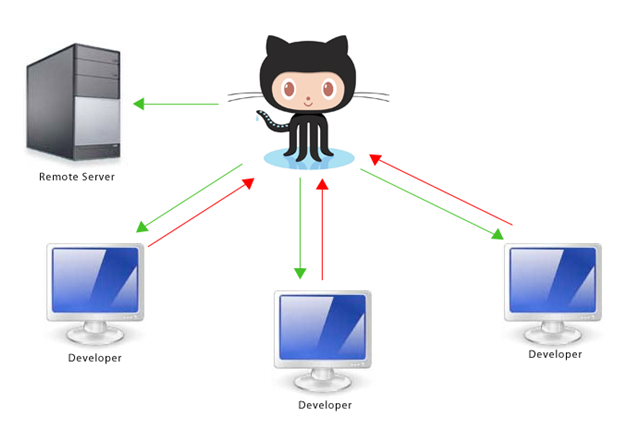
\includegraphics[width=0.5\textwidth]{Images/2}
\end{figure}

}

    \frame{
        \frametitle{Instalar Git}

        \begin{itemize}

                \item Windows
                      \begin{itemize}
                      \item Git Bash
                                  \begin{enumerate}
                                  \item Ir a http://git-scm.com/download/win
                                  \item Instalar
                            \end{enumerate}
                \item Plug-in IDE
                \end{itemize}

        \item Linux
        \begin{enumerate}
        \item Entrar a la terminal
        \item Digitar ``sudo apt-get install git-all'' 
        \end{enumerate}

        \end{itemize}

\begin{figure}[t]
    \centering
    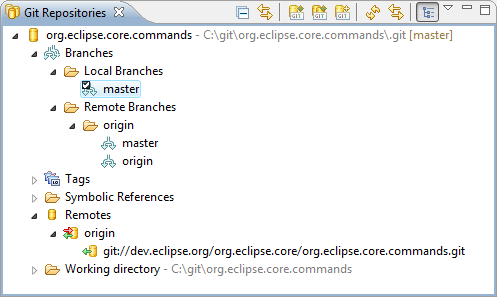
\includegraphics[width=0.5\textwidth]{Images/3}
\end{figure}
}

    \frame{
\frametitle{C\'omo crear un repositorio}
 % como se crea el repositorio
\begin{enumerate}
\item Creamos el directorio  (mkdir) 
\item Desde la terminal nos ubicamos en el directorio (cd)
\item Digitamos "git init"
\end{enumerate}

Si ya habíamos creado el repositorio podemos clonarlo.Ubicados en el directorio, digitamos "git clone [URL del repositorio]".

\begin{figure}[t]
    \centering
    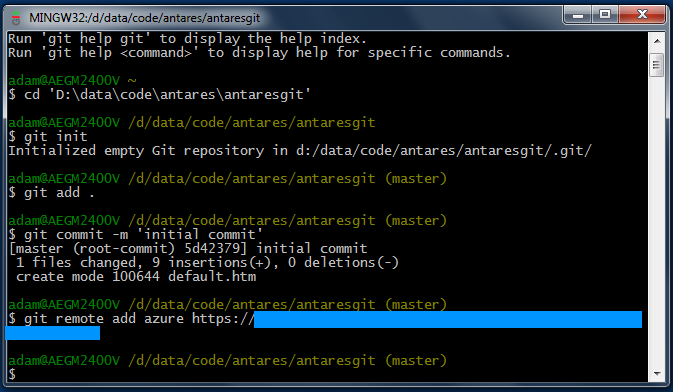
\includegraphics[width=0.5\textwidth]{Images/4}
\end{figure}
}

    \frame{
  \frametitle{Los tres estados} 
  Git tiene tres estados principales, que tus archivos pueden poseer:
  \begin{itemize}
  \item Commited: Guardado sin peligro en tu repositorio.
  \item Modified: El archivo tiene cambios, pero no se ha agregado.
  \item Staged: Agregado, pero no se ha hecho el commit al repositorio.
  \end{itemize}

  Esto nos conduce tambi\'en a las tres principales secciones de Git: 
       
\begin{figure}[t]
    \centering
    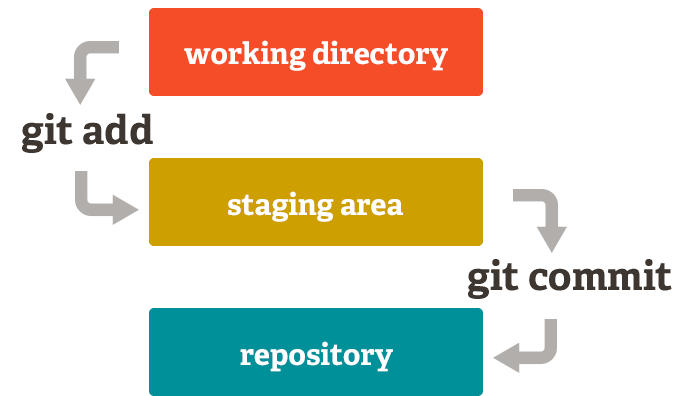
\includegraphics[width=0.5\textwidth]{Images/5}
\end{figure}
  }    

    \frame{
\frametitle{Principales conceptos}

% Aqui vamos a poner los principales comandos o conceptos, falta explicarlos
\begin{itemize}
\item git status
\item git commit
\item git add %añadir el archivo
\item git log %listado de commits
\item git branch %listado de ramas
\item reset

\end{itemize}


}
    \section{C\'omo compartir un repositorio?}
    \begin{frame}[fragile]
    \frametitle{Definiciones}
    \begin{alertblock}{Fork:}
        Es una copia exacta de un repositorio, sin embargo tendremos\\
        dos repositorios independientes, con diferente URL que pueden\\
        cada uno evolucionar de forma totalmente aut\'onoma. \\
    \end{alertblock}

    \begin{alertblock}{Repositorio upstream:}
        Es el repositorio original; no podremos hacer ning\'un cambio\\
        directamente sobre este repositorio, ya que no tendremos permisos\\
        de escritura sobre el mismo. Lo que haremos es crear nuestra propia\\
        copia (fork) del mismo.
    \end{alertblock}
\end{frame}

\begin{frame}[fragile]
    \frametitle{Definiciones}
    \begin{alertblock}{Repositorio origin:}
        Es nuestra copia del repositorio que forkeamos alojada en github.\\
        A este repositorio enviaremos los cambios que efectuaremos en nuestro
        \\repositorio local.
    \end{alertblock}

    \begin{alertblock}{Repositorio local:}
        Es el repositorio local que tendremos en nuestra propia estaci\'on 
        de\\trabajo.
    \end{alertblock}
\end{frame}

\begin{frame}[fragile]
    \frametitle{Compartir Repositorio}
    \textbf{1.Hacer un Fork}\\
        Del repositorio upstream, del que haremos copia, de esta forma ya 
        tendremos nuestro repositorio origin.
        \begin{figure}[t]
            \raggedleft
            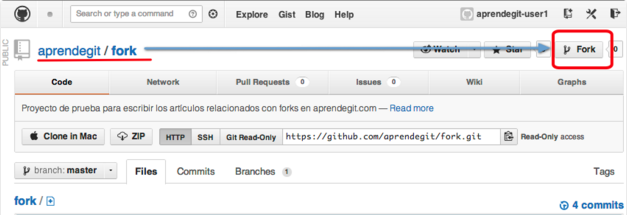
\includegraphics[width=1\textwidth]{Images/6.png}
        \end{figure}
\end{frame}

\begin{frame}[fragile]
    \frametitle{Compartir Repositorio}
    \textbf{2.Clonar repositorio origin en un repositorio local}
    \begin{figure}
        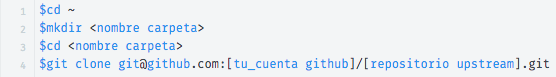
\includegraphics[width=1\textwidth]{Images/7.png}
    \end{figure}

    \textbf{3.Guardar Cambios}
    \begin{figure}
        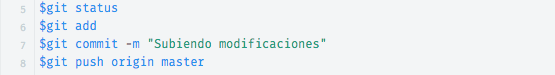
\includegraphics[width=1\textwidth]{Images/8.png}
    \end{figure}
\end{frame}

\begin{frame}[fragile]
    \frametitle{Mantener Repositorios Actualizados}
    Configurar el repositorio upstream como un repositorio remoto (remote)
    vinculado a nuestro repositorio local.Situados en el directorio del 
    repositorio, deberemos ejecutar:
    \begin{figure}
        
\includegraphics[width=1\textwidth]{Images/9.png}
    \end{figure}
    Cuando querramos traer las actualizaciones de upstream, deberemos 
    ejecutar:
    \begin{figure}
        
\includegraphics[width=1\textwidth]{Images/10.png}
    \end{figure}
\end{frame}

    \section{Committing, Pull y Push}
    \begin{frame}[fragile]
    \frametitle{Haciendo Commit}
    En GitHub, cuando se guardan cambios se le llama \alert{commits}.\\
    Cada confirmaci\'on se le asociado un mensaje de confirmaci\'on, \\
    que es una descripci\'on que explica por qué se hizo un cambio en\\
    particular.
    \begin{figure}
        
\includegraphics[width=1\textwidth]{Images/11.png}
    \end{figure}
    Para obtener informaci\'on sobre el estado de nuestro repositorio\\
    usaremos el comando \alert{git status}.
    \begin{figure}
        
\includegraphics[width=1\textwidth]{Images/12.png}
   \end{figure}
\end{frame}

    \begin{frame}[fragile]
    \frametitle{Haciendo Pull}
    Para actualizar tu repositorio local al commit m\'as nuevo, ejecuta\\
    \alert{git pull} en tu directorio de trabajo para \textbf{bajar} y \textbf{fusionar} los cambios remotos. Al ejecutar \textbf{git pull}, por lo general
    se recupera la informaci\'on del servidor del que clonaste, y 
    autom\'aticamente se intenta unir con el c\'odigo con el que est\'as 
    trabajando actualmente.
\end{frame}

    \begin{frame}[fragile]
    \frametitle{Haciendo Push}
     Cuando tu proyecto se encuentra en un estado que quieres compartir,
     tienes que enviarlo a un repositorio remoto. El comando que te permite 
     hacer esto es:\\
     \alert{git push [nombre-remoto][nombre-rama]}. \\Si quieres
     enviar tu rama maestra (master) a tu servidor origen (origin), se 
     ejecuta el comando \alert{git push origin master} para enviar tu 
     trabajo al servidor: \\
     \alert{git push origin master}
\end{frame}

    \section{C\'omo crear un Branch?}
    \begin{frame}[fragile]
    \frametitle{C\'omo crear un branch?}
    ¿y qu\'e es un branch?. La traducci\'on literal ser\'ia: rama.
    Es decir, dentro de nuestro sistema de control de versiones podemos ver
    el hist\'orico de cambios como si de un \'arbol se tratase. 
    De esta forma podemos ir abriendo ramas que parten bien de la rama 
    principal (master) o de otra rama (branch).
    \begin{figure}
        
\includegraphics[width=1\textwidth]{Images/13.png}
    \end{figure}
    Con esto creamos un branch y con el checkout nos movemos a \'el 
    (el working directory queda apuntando a este branch para poder trabajar 
     con el).
\end{frame}

\begin{frame}[fragile]
    \frametitle{Visualiar los Branch que tenemos}
    Ejecutamos el comandos \alert{git branch} y obtendremos una salida de 
    este estilo:
    \begin{figure}
        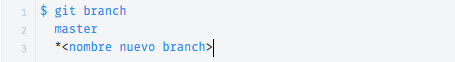
\includegraphics[width=1\textwidth]{Images/14.png}
    \end{figure}
    Donde el \'* indica el branch activo. El listado anterior solo muestra 
    los branch locales, pero tambi\'en podemos listar los branch remotos si 
    hacemos: \alert{git branch -a}.
\end{frame}

    \section{Branching y Merging}
    \begin{frame}[fragile]
    \frametitle{Haciendo Merging}
    Para fusionar otra rama a tu rama activa (por ejemplo master), utiliza el
    comando \alert{git merge [branch]}. En ambos casos git intentar\'a
    fusionar autom\'aticamente los cambios. Desafortunadamente, no siempre 
    ser\'a posible y se podr\'an producir conflictos. 
    Tú eres responsable de fusionar esos conflictos manualmente al editar los
    archivos mostrados por git. Despu\'es de modificarlos, necesitas 
    marcarlos como fusionados con el comando \alert{git add [nombre archivo]}
\end{frame}


\end{document}
